\section{Кеширование. Cache-Aside и Cache-Through архитектуры, слабые модели консистентности}
    Главная мотивация - уменьшение задержки, также - сглаживание нагрузки, популярные объекты будут часто запрашиваться из кеша. \\
    Поэтому нагрузка на базу данных будет распределена более равномерно.\\
    Задержка при чтении из кеша маленькая, поскольку:\\
    \begin{itemize}
      \item Кеш обычно держит все данные в RAM.
      \item Кеш не поддерживает персистентность.
      \item Кеш не поддерживает сложные индексы (почти все кеш - просто хеш-таблица).
    \end{itemize}
    Архитектуры кеша:
    \begin{itemize}
        \item Cache-Aside - кеш и СУБД напрямую не общаются, клиент делает запросы и туда, и туда. (Пример - MySQL + Memcached).\\
        \begin{figure}[h]
            \centering
            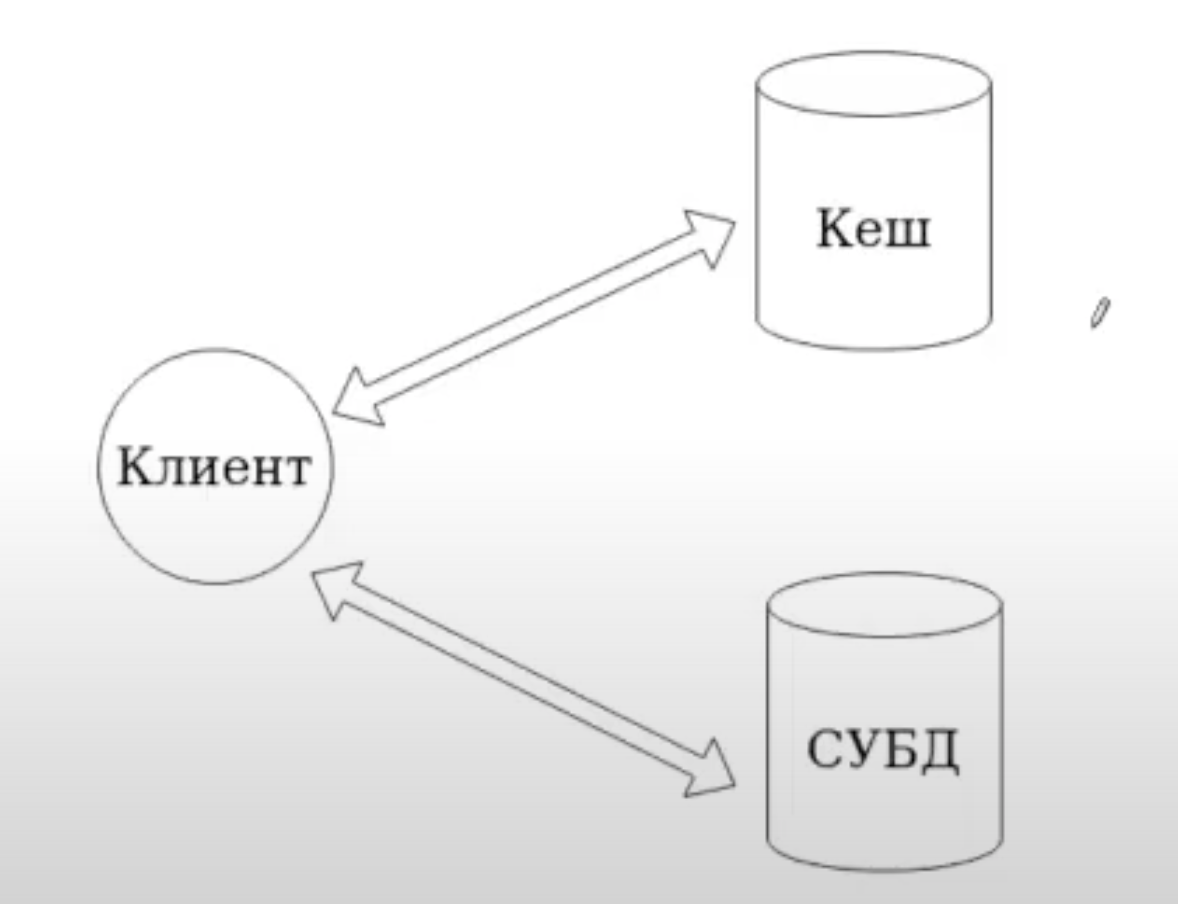
\includegraphics[scale = 0.5]{18.png}
            \caption{}
        \end{figure}
        \begin{itemize}
            \item синхронные запросы - спросить в кеше, если там нет, спросить в базе данных и записать в кеш \\
            Время на запрос при отсутствии значения в кеше: $2 * RTT(cache) + RTT(DB)$\\
            \begin{figure}[h]
                \centering
                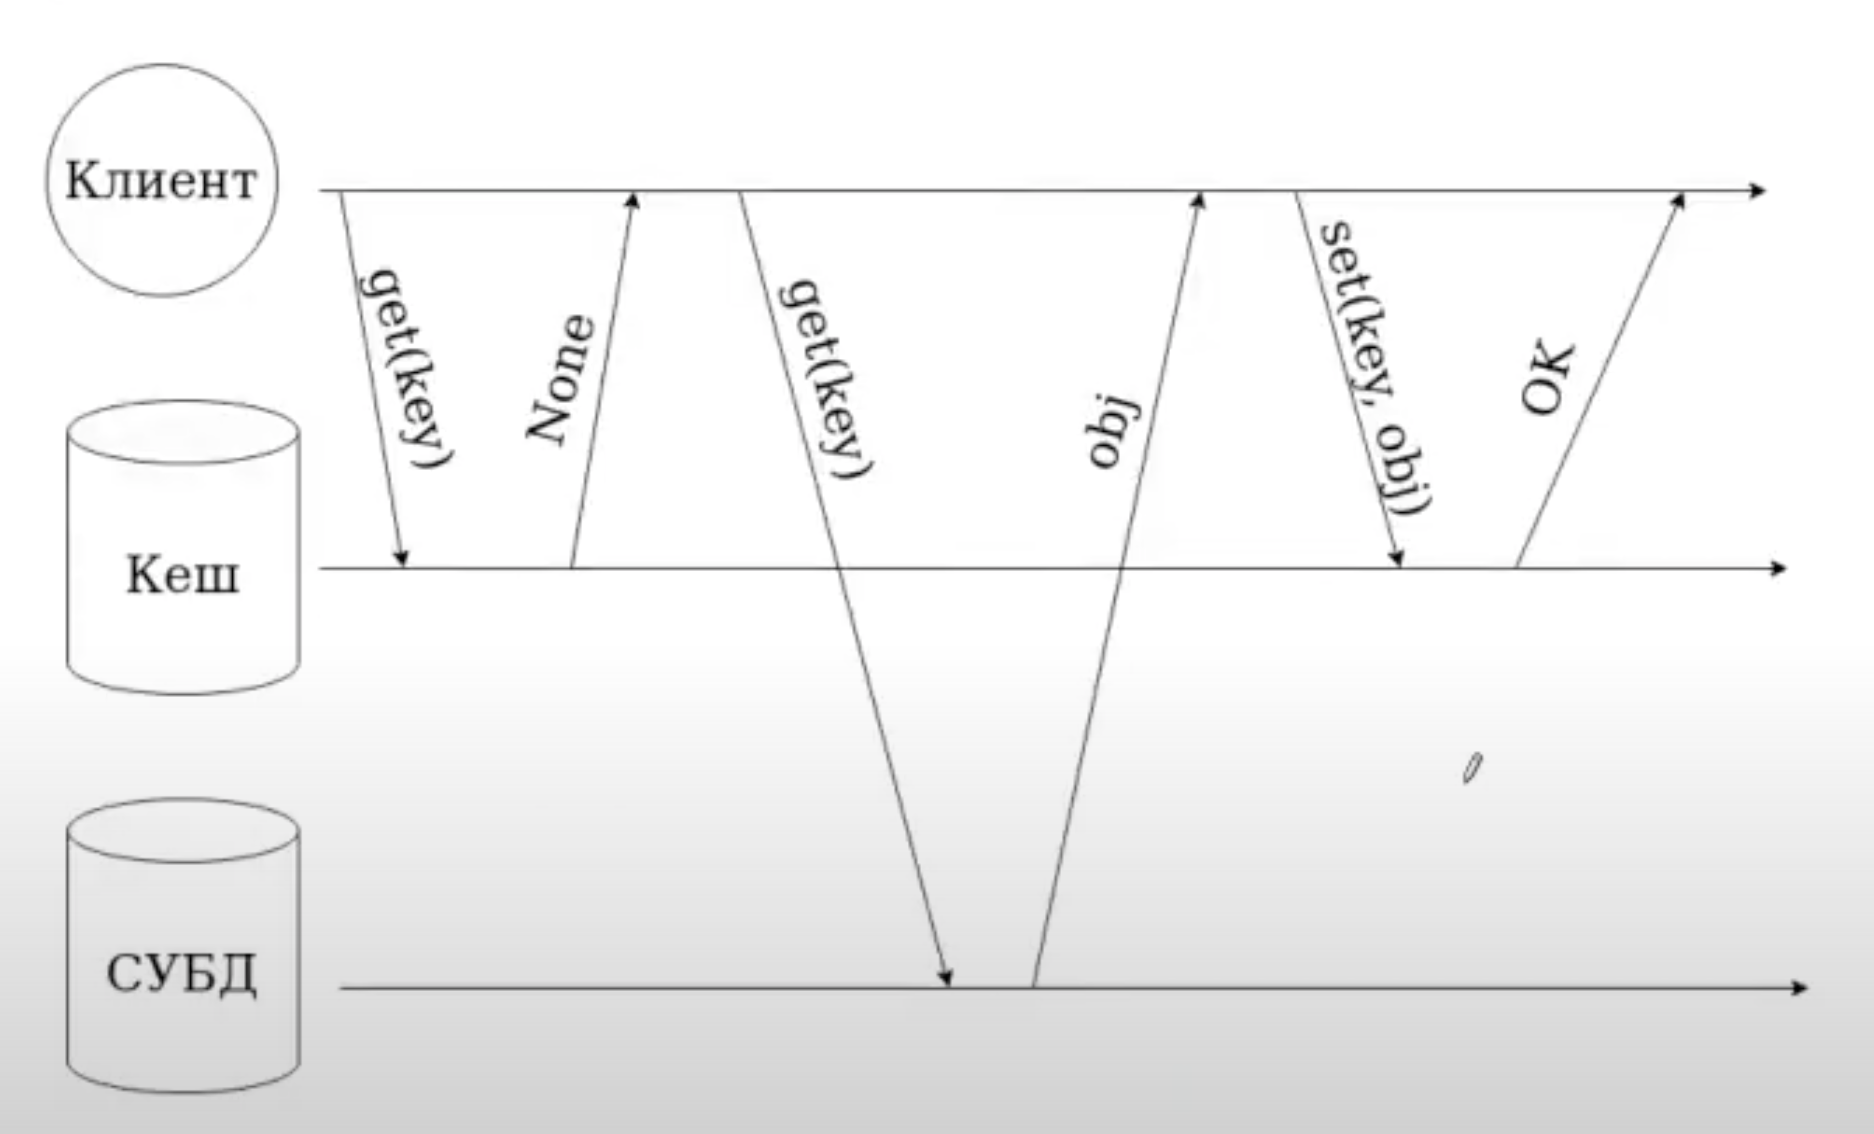
\includegraphics[scale = 0.5]{19.png}
                \caption{}
            \end{figure}
            \item асинхронный запрос - делаем запрос одновременно и в кеш и СУБД \\
            Время на запрос при отсутствии значения в кеше получим ответ быстрее: $RTT(cache) + RTT(DB)$, но тратим пропускную способность СУБД впустую, если значение есть в кеше.\\
            \begin{figure}[h]
                \centering
                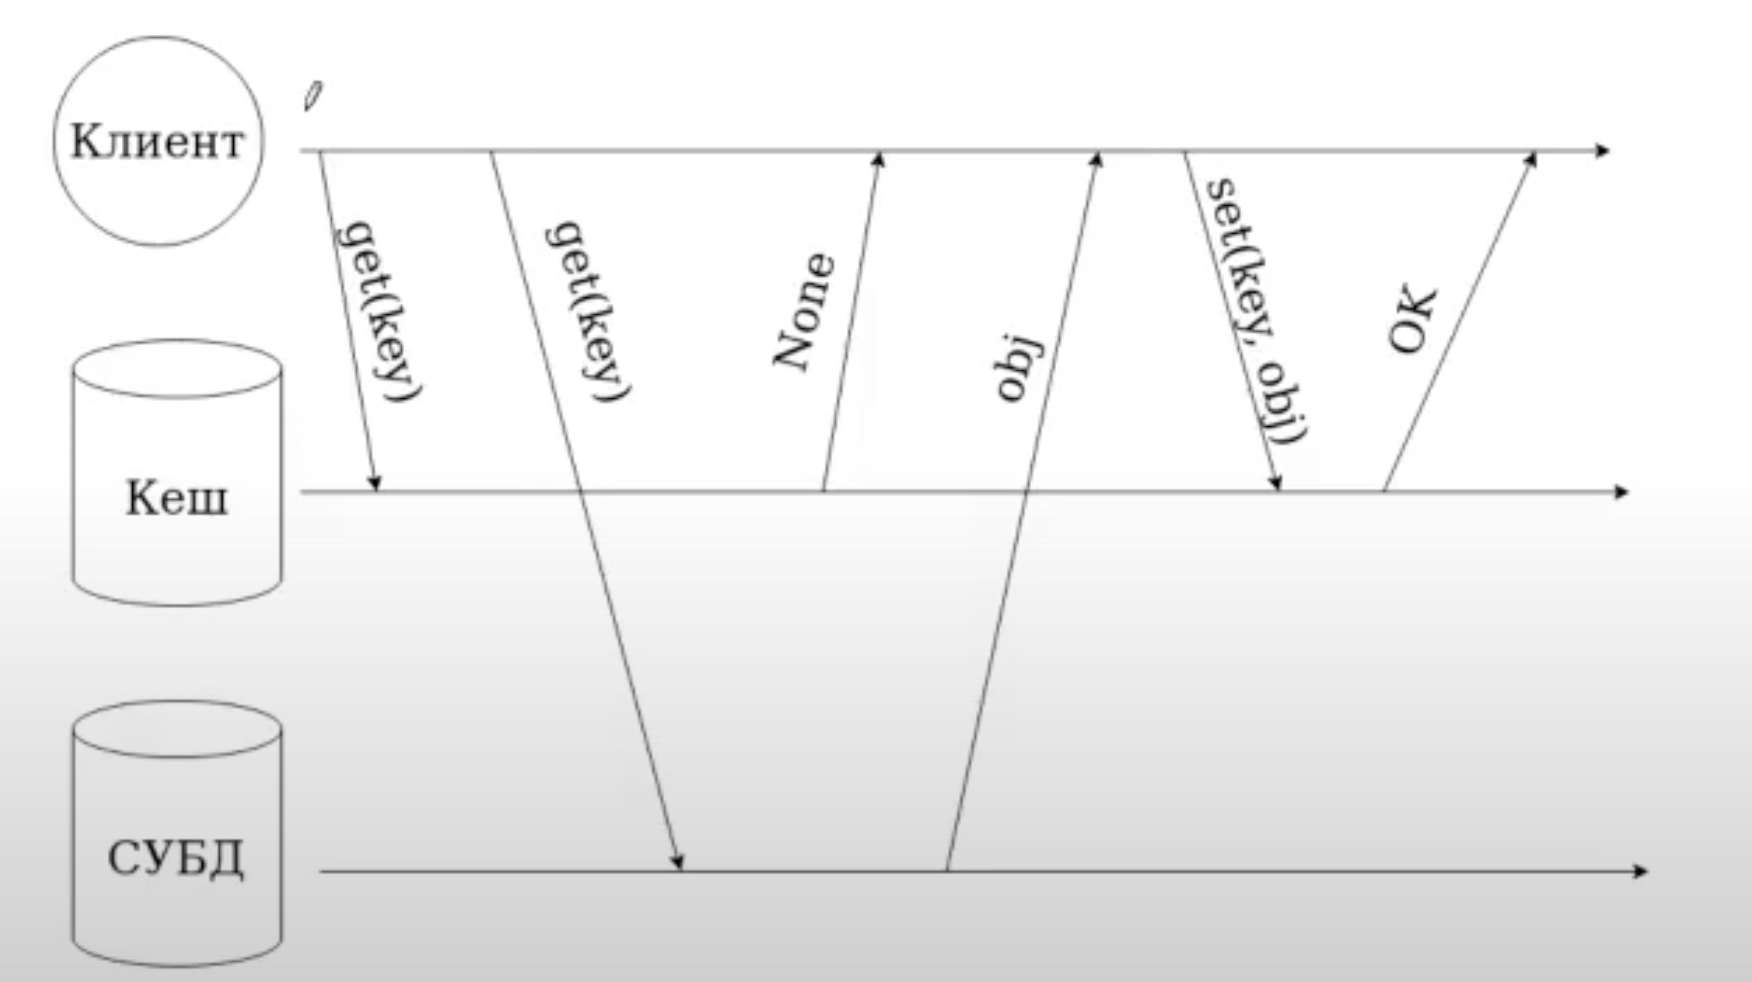
\includegraphics[scale = 0.5]{20.png}
                \caption{}
            \end{figure}
        \end{itemize}
        Если мы произвели запись в СУБД, затем клиент умер и мы не успели записать значение в кеш, в кеше сохранится устаревшее значение. \\
        Решение - добавим TTL, чтобы удалять старые значения.\\
        \begin{figure}[h]
            \centering
            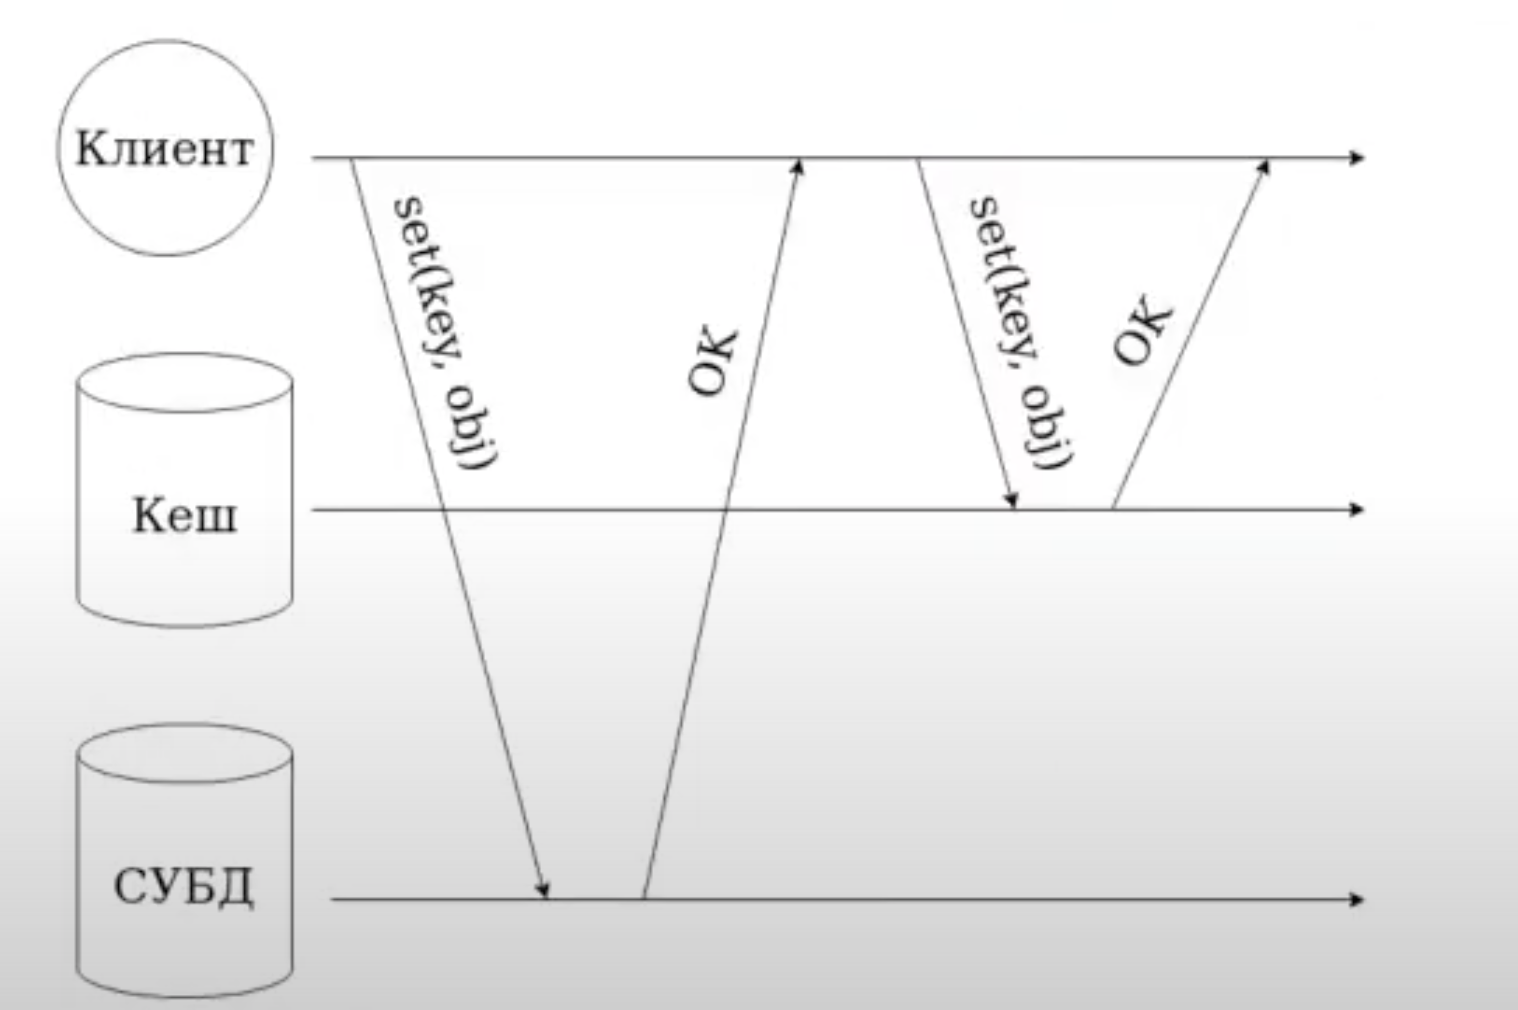
\includegraphics[scale = 0.5]{21.png}
            \caption{}
        \end{figure}
        \item Cache-Through - клиент обращается к кеш + СУБД как к единому целому. \\
        Время на запрос при отсутствии значения в кеше: $RTT(cache) + RTT(DB)$ и СУБД обслуживает только те запросы, которых нет в кеше (пропускная способность не тратится напрасно) \\
        \begin{figure}[h]
            \centering
            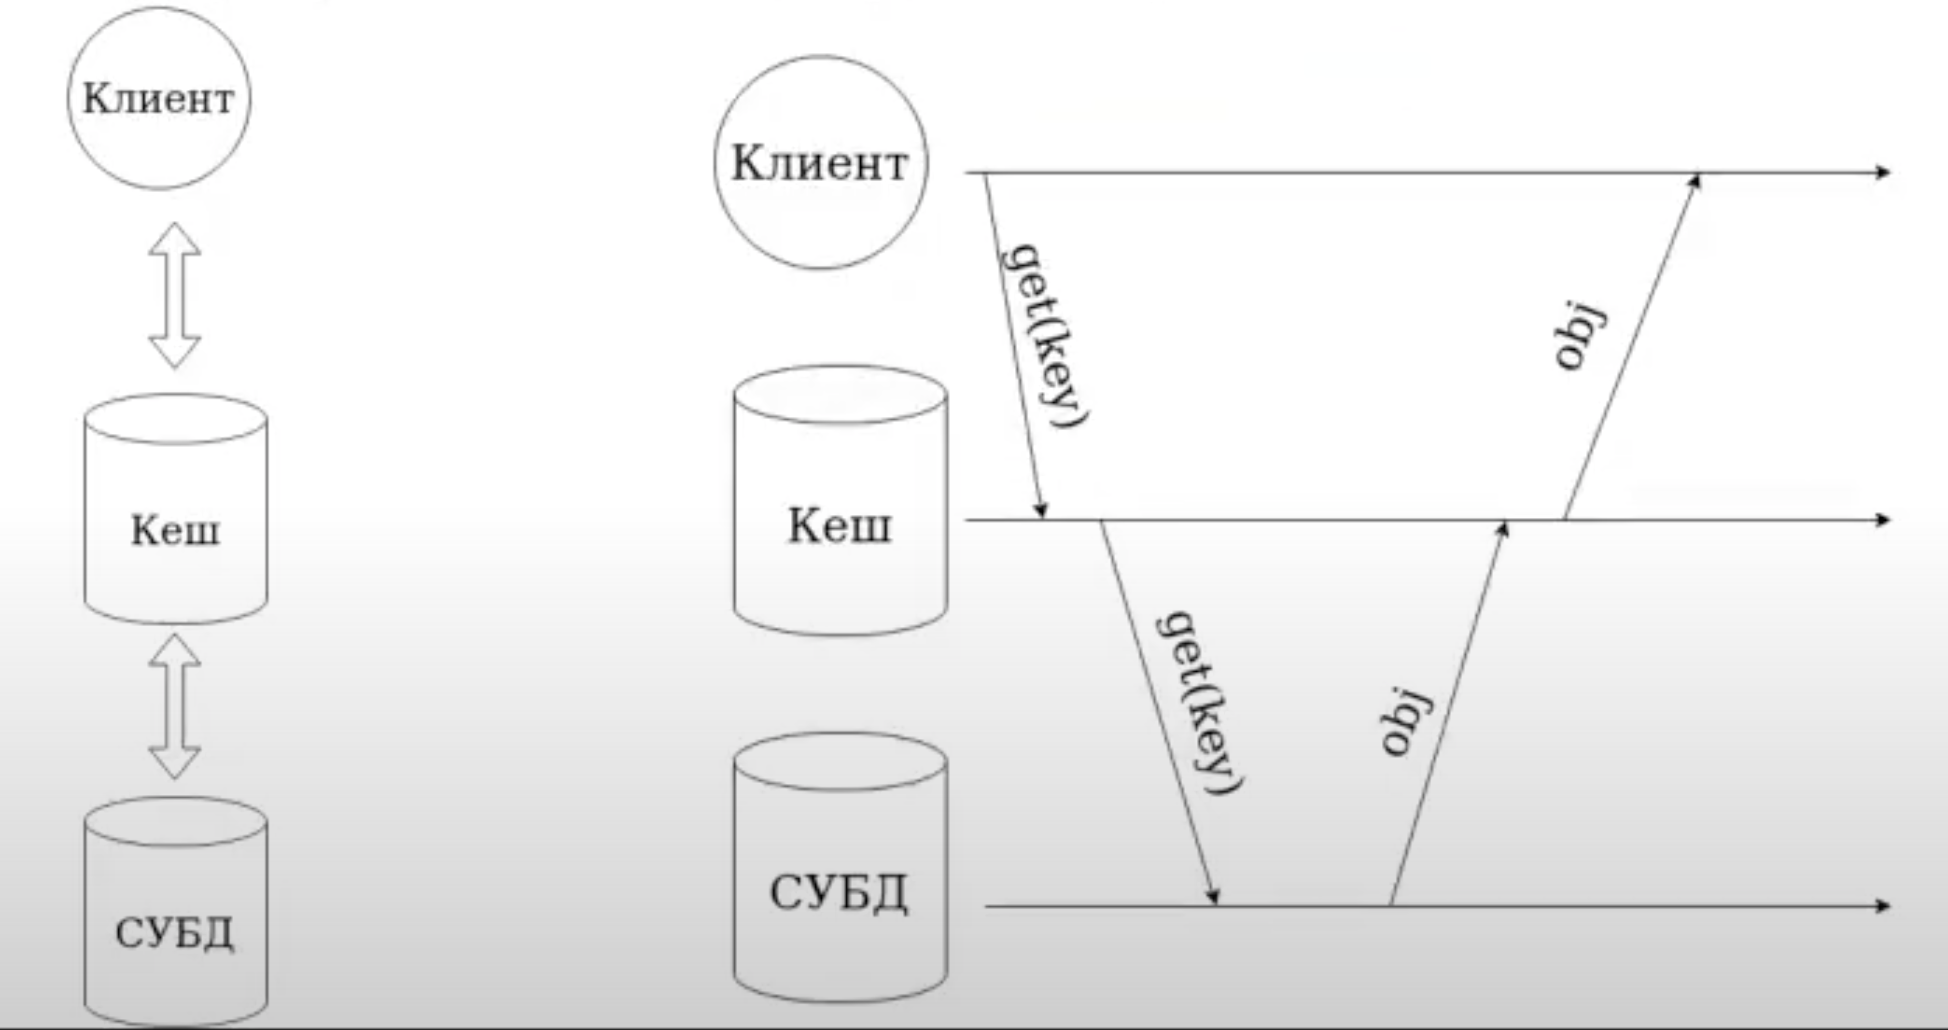
\includegraphics[scale = 0.5]{22.png}
            \caption{}
        \end{figure}
        Также СУБД может самостоятельно наполнять кеш результатами популярных запросов.
    \end{itemize}

    \subsection{Кеширование и слабые модели консистентности}
    Можно думать о кешах как о асинхронных репликах, в которых есть все те же проблемы и такие же способы их решения: чтение собственных изменений - читаем данные которые мы можем изменить из СУБД, без использования кеша, монотонное чтение - читаем из одного и того же кеша. \\
    Можно ли записывать в кеш - это снизит задержку на запись (в СУБД будем писать только когда кеш переполнится), но жертвуем Durability (кеш подтвержил клиенту запись, но упал и значения из RAM'а потерялись).\\
    Если кешей, поддерживающих запись, несколько - будем думать о таких системах как о Multi-Leader Replication. \\
    \subsection{Определение несуществования объекта в СУБД с помощью кеша}
    Будем кешировать подотрезок, отсортированного отрезка, который хранится в СУБД, по этому подотрезку можно понять отсутствие некоторых элементов в субд.\\
    Пример:\\
    \begin{figure}[h]
        \centering
        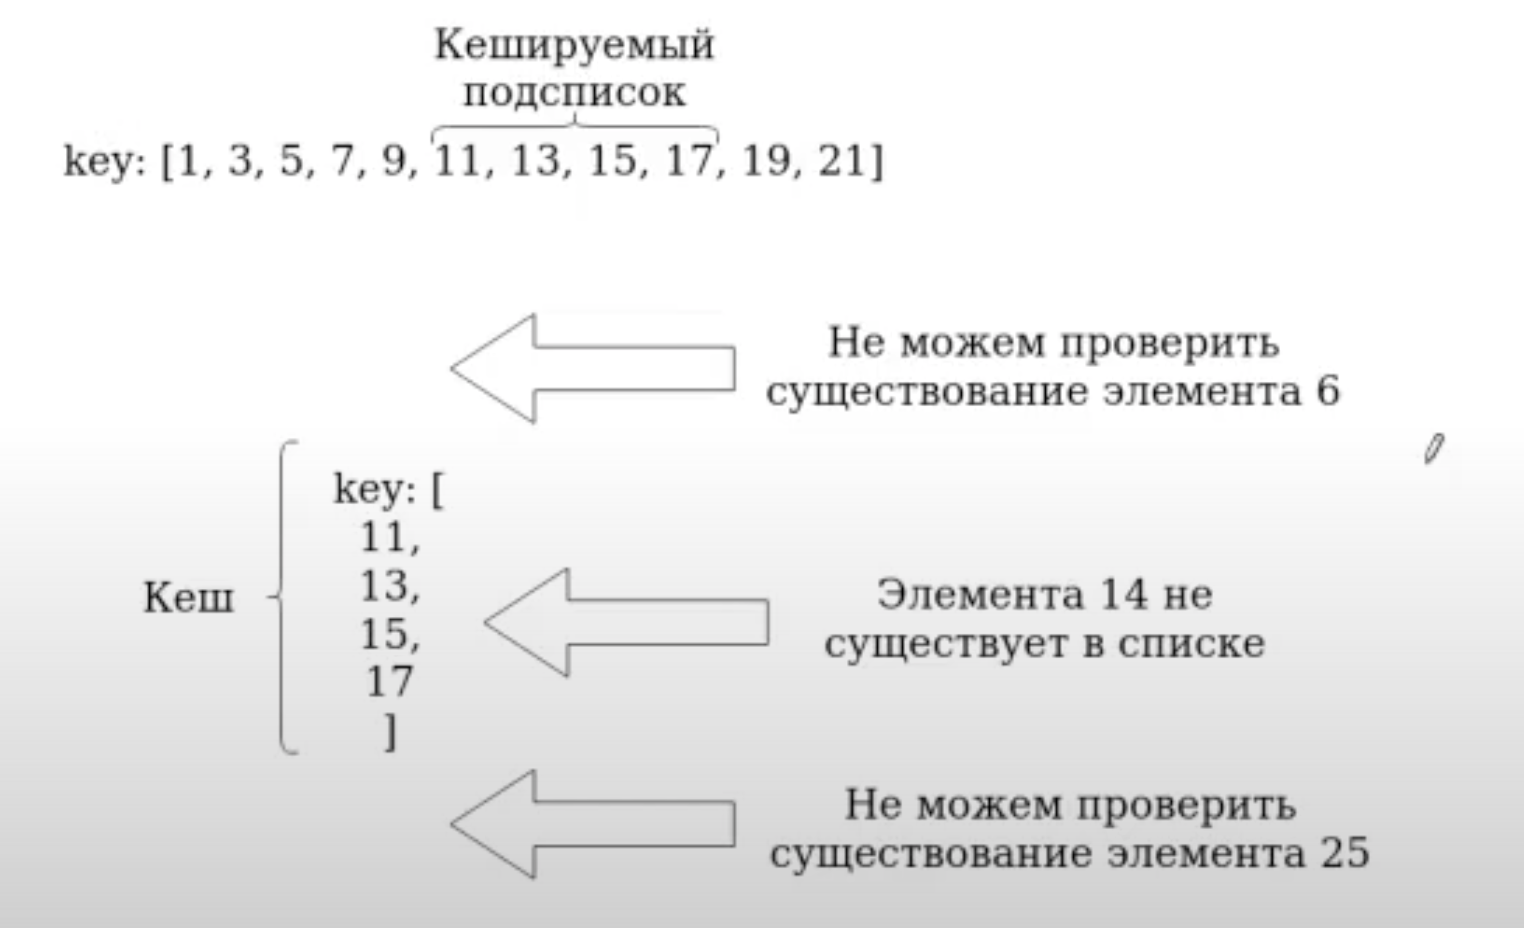
\includegraphics[scale = 0.5]{23.png}
        \caption{}
    \end{figure}
